% ===============================

\section{Case Study}\label{sec:case-studies}
    In this section I detail the intermediate outputs of the index construction for the GP \textit{TPG}.
    For this GP, 810 documents have been processed, including the document I will pick as an example, \textit{1047 - Oregon Public Employees Retirement Fund Opportunity Portfolio}, which details the performance of several funds in which the Oregon Public Employees Retirement Fund is invested, managed by TPG\@.
    The first step of the elaboration is the summary, which I present below as produced by the model:

    \begin{lstlisting}[style=cmd, label={lst:oregon_summary}]
        ### Summary of Investment Report (Focusing on TPG's Perspective)

        The report provides an overview of several private equity partnerships managed by TPG, including the TPG Opportunity Fund (I), TPG Specialty Lending Fund, and TPG Specialties LP. Below is a summary of each fund's performance as of December 31, 2020:

        #### **TPG Opportunity Fund (I)**
        - **Total Value Multiple**: 1.43x
        - **Time-Weighted Return (TWR)**: 6.1%
        - **Performance Perspective**: The fund is performing well with a strong total value multiple and modest growth rate.

        #### **TPG Specialty Lending Fund**
        - **Total Value Multiple**: 2.75x
        - **Time-Weighted Return (TWR)**: 15.0%
        - **Performance Perspective**: The fund shows significant upside potential, driven by favorable performance in its loan portfolio.

        #### **TPG Specialties LP**
        - **Total Value Multiple**: 1.38x
        - **Time-Weighted Return (TWR)**: 8.0%
        - **Performance Perspective**: The fund has modest growth but is lagging compared to the Specialty Lending Funds due to lower-than-expected performance in some of its loan portfolio.

        ### Manager's Perspective on Capital Distributions

        TPG's manager believes that capital distributions for the year following the report date (2021) will vary across funds based on their current performance and structural characteristics:

        1. **TPG Opportunity Fund (I)**: The fund is expected to receive moderate capital distributions, commensurate with its strong performance. TPG anticipates that the fund's capital distribution timing aligns closely with its performance momentum.

        2. **TPG Specialty Lending Funds**: These funds are projected to experience higher capital distributions due to their significant upside potential and favorable loan portfolio performance. TPG expects these funds to maintain their leading position in terms of capital distribution magnitude.

        3. **TPG Specialties LP**: The fund is expected to receive lower capital distributions compared to the Specialty Lending Funds, reflecting its modest growth trajectory.

        ### Confidence Level

        - **For TPG Opportunity Fund (I)**: High confidence due to strong performance and stability.
        - **For TPG Specialty Lending Funds**: Very high confidence given their favorable loan portfolio performance.
        - **For TPG Specialties LP**: Moderate confidence due to lower upside potential compared to the Specialty Lending Funds.

        ### Conclusion

        TPG anticipates that capital distributions will be distributed in a manner that reflects each fund's current performance. The manager is optimistic about the opportunities for growth across all funds but acknowledges that diversification among these funds could lead to varying distribution timings and magnitudes.

        This summary provides TPG's perspective on its investment strategy, emphasizing the importance of managing multiple private equity partnerships with different performance characteristics to achieve steady capital distribution outcomes in 2021.
    \end{lstlisting}
    
	The output of the first phase is then fed once again to the model, to produce the following JSON output:
    
	\begin{lstlisting}[style=json,label={lst:TPG_results}]
    {
      "results": [
        {
          "fund_name": "TPG Opportunity Fund (I)",
          "report_date": "2021",
          "outlook": "increase",
          "magnitude": 5,
          "confidence": 0.8,
          "explanation": "The fund is expected to receive moderate capital distributions due to its strong performance momentum."
        },
        {
          "fund_name": "TPG Specialty Lending Fund",
          "report_date": "2021",
          "outlook": "increase",
          "magnitude": 10,
          "confidence": 0.95,
          "explanation": "The fund is projected to experience higher capital distributions due to its significant upside potential."
        },
        {
          "fund_name": "TPG Specialties LP",
          "report_date": "2021",
          "outlook": "increase",
          "magnitude": 4,
          "confidence": 0.6,
          "explanation": "The fund is expected to receive lower capital distributions due to its modest growth trajectory."
        }
      ]
    }
    \end{lstlisting}

    Then, all the entries from the JSON files are compiled in a database, for a total of 880 entries, as most documents focus on a single fund and some do not contain relevant information.
    After aggregation, index shown in Fig. \ref{fig:21_TPG} is produced:
    \begin{figure}[h!]
		\centering
        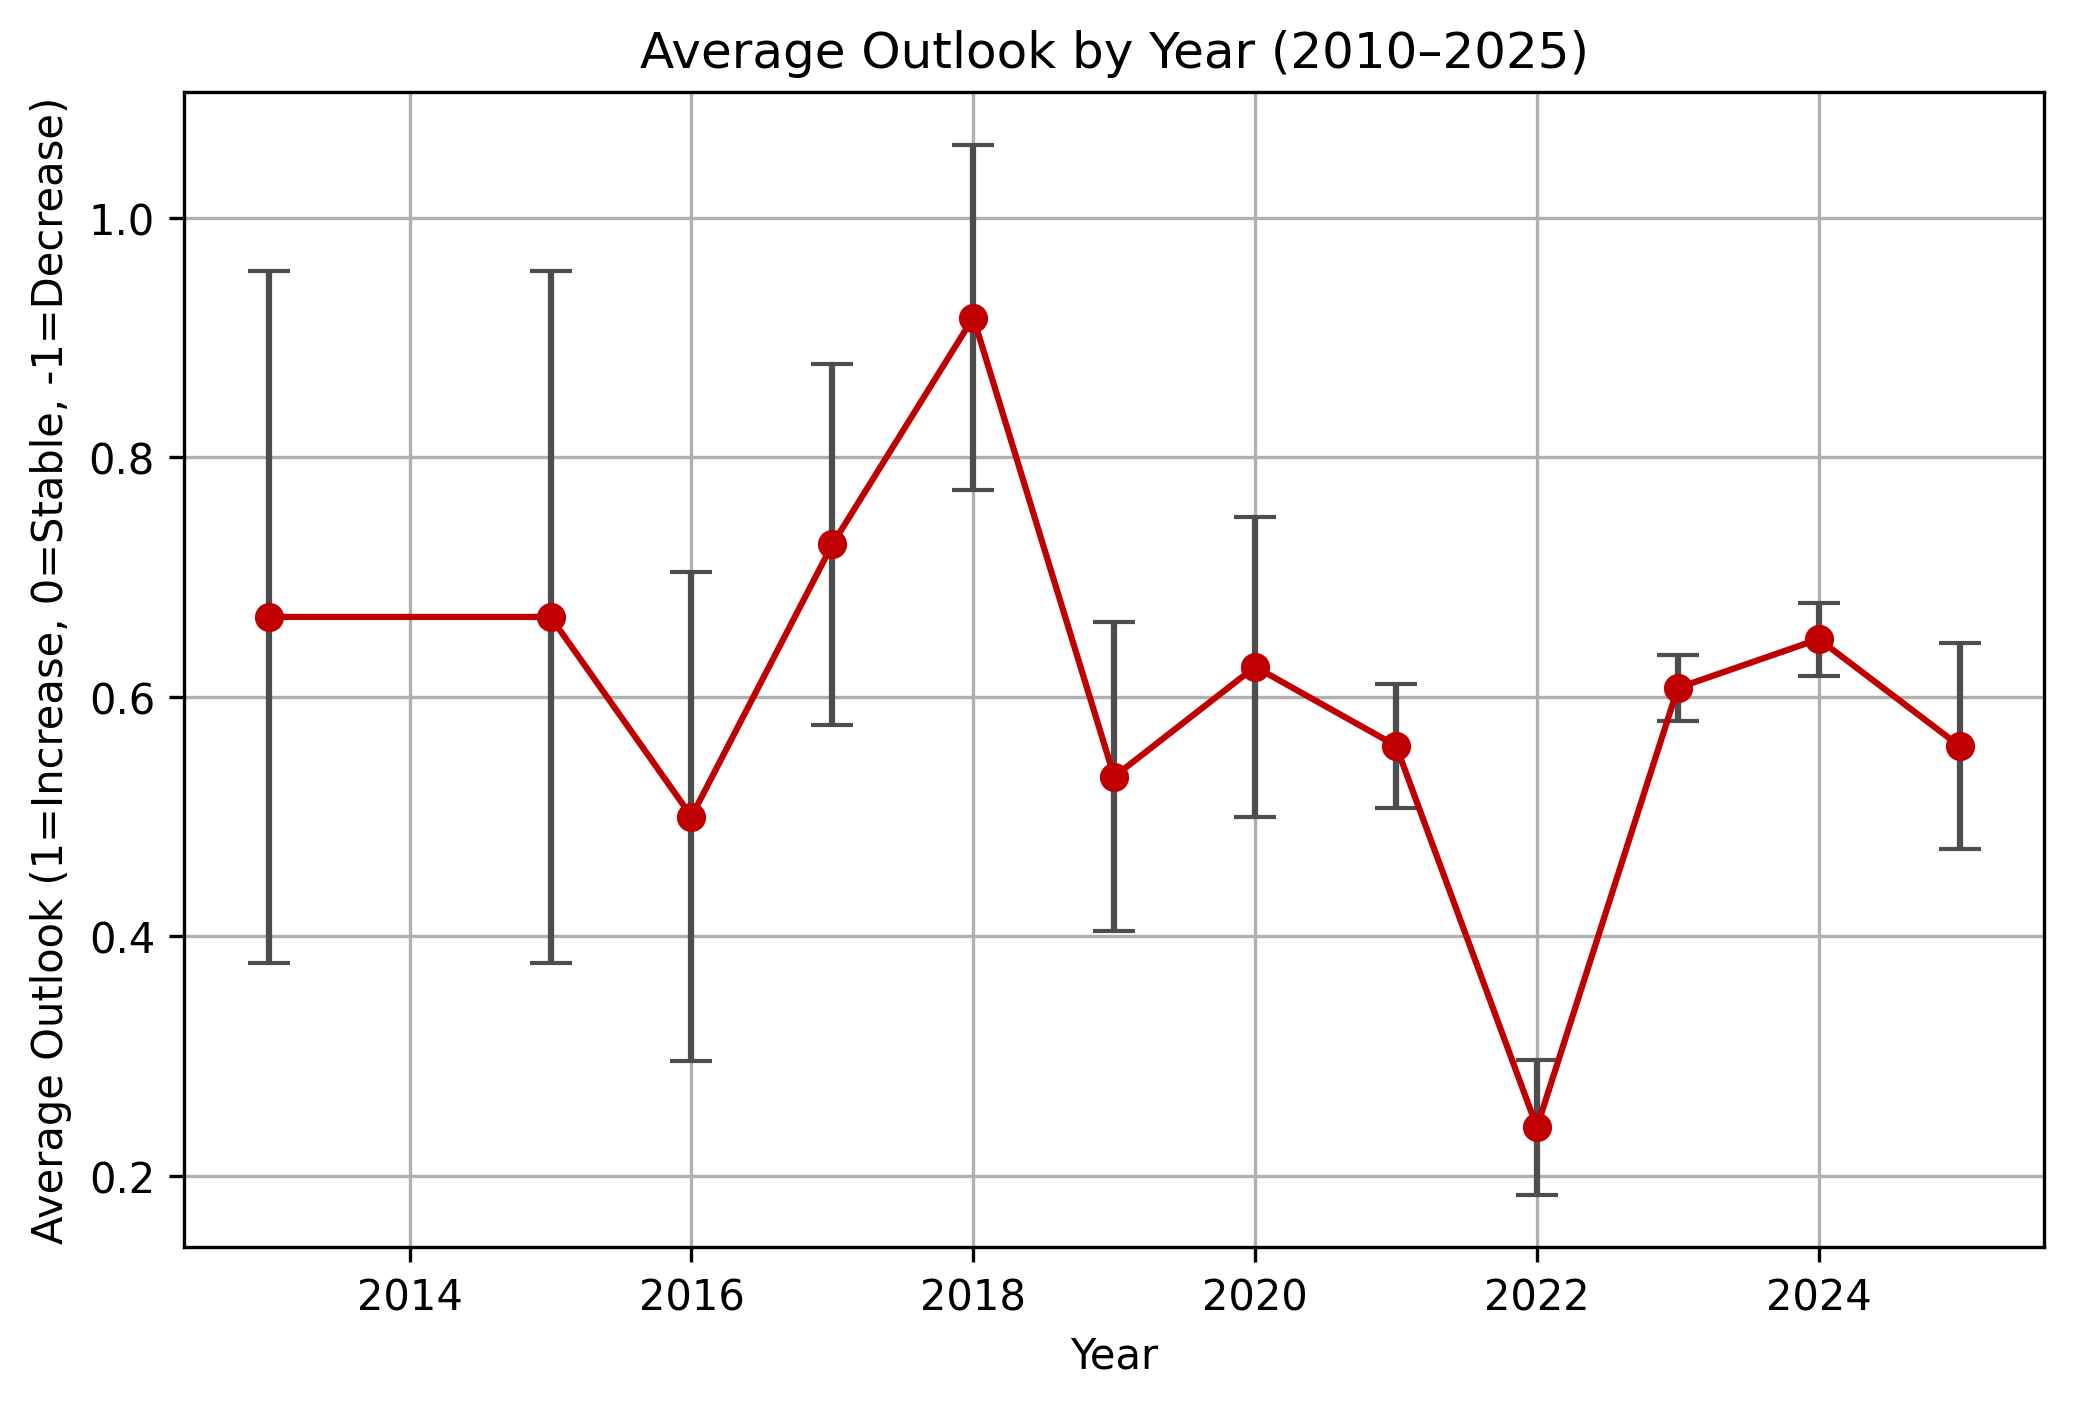
\includegraphics[width=0.7\linewidth]{img/21_TPG}
        \caption{Quarterly aggregation for the sentiment index for the \textit{TPG} GP. Error bar sizes are inversely proportional to the number of available data entries for each quarterly point.}
        \label{fig:21_TPG}
    \end{figure}

    Finally, after filtering points with too few observations, an OLS regression is run on the actual data that the index is meant to represent.
    The results of the regression using yearly aggregation, reported in Table~\ref{tab:ols_sentiment}, show a considerable and significant collinearity between the index and the actual data.

    \begin{table}[h!]
        \centering
        \begin{tabular}{lcccc}
        \toprule
         & Coef.
         & Std.
         Err.
         & t & P$>|t|$ \\
        \midrule
        \textbf{const} & 0.6471 & 0.037 & 17.614 & 0.000 \\
        \textbf{rel\_change\_net\_cf} & 0.5885 & 0.117 & 5.038 & 0.015 \\
        \midrule
        \multicolumn{5}{l}{\textit{Observations}: 5, \quad \textit{R$^2$}: 0.894, \quad \textit{Adj. R$^2$}: 0.859} \\
        \multicolumn{5}{l}{\textit{F-statistic}: 25.38 (p = 0.015), \quad \textit{DW}: 1.873} \\
        \bottomrule
        \end{tabular}
        \caption{OLS Regression of Sentiment on Net Cashflow Changes}
        \label{tab:ols_sentiment}
    \end{table}

    \begin{figure}
        \centering
        \includegraphics[width = 0.7\linewidth]{img/21_TPG_Lagged Sentiment vs Relative Change in Net Cashflow (TPG)}\\
        \caption{Comparison between the sentiment index and the data from Preqin}
        \label{fig:sentiment_TPG}
    \end{figure}

\section{Panel Regression}

\section{Confidence of Results}
    \begin{figure}
        \centering
        \includegraphics[width = 0.4\linewidth]{img/21_TPG_outlook_distribution} \quad
        \includegraphics[width = 0.4\linewidth]{img/23_AGM_outlook_distribution}
        \caption{Distribution of outlooks and confidence levels for funds TPG and Apollo Global Management}
        \label{fig:confidence}
    \end{figure}
It can be observed from the distribution of the outlooks and the of the confidence values that, despite majority of the forecasts expect a positive outlook, the confidence of the model in his forecasts remains very low, with the $0-10\%$ confidence bucket taking the majority of observations (ref. Fig. \ref{fig:confidence})


\section{Comparison with Market Baselines}\label{sec:comparison-with-public-market-baselines}

A primary concern is the potential presence of look-ahead bias, meaning the language model may have been trained on the same information later used to construct the sentiment index.
While it is highly unlikely that the model was trained on proprietary Preqin documents, its forecasts could still be influenced by publicly available information covering similar content.
To address this concern, an initial test was conducted by regressing the sentiment index on macroeconomic variables—factors that are almost certainly part of the model's training data.
The results showed no significant correlation (see Table~\ref{tab:ols_market}), suggesting that the index does not simply reflect pre-existing knowledge of macro trends.


\begin{table}[H]
        \centering
        \caption{OLS Regression Results}
        \begin{tabular}{lccc}
        \toprule
        \textbf{Variable} & \textbf{Coefficient} & \textbf{Std. Error} & \textbf{t-Stat (p-value)} \\
        \midrule
        \textbf{const}   & 0.7880 & 0.112  & 7.005 \; (0.000) \\
        \textbf{snp500}  & 0.4859 & 0.495  & 0.981 \; (0.348) \\
        \textbf{irr}     & -1.2399 & 0.820 & -1.513 \; (0.159) \\
        \midrule
        \multicolumn{4}{l}{\textbf{Model Statistics:}} \\
        \multicolumn{4}{l}{R-squared: 0.173 \quad Adj. R-squared: 0.023} \\
        \multicolumn{4}{l}{F-statistic: 1.153 \quad Prob(F-statistic): 0.351} \\
        \multicolumn{4}{l}{Observations: 14 \quad Durbin-Watson: 1.398} \\
        \bottomrule
        \end{tabular}
        \label{tab:ols_market}
    \end{table}



% ===============================